%
% teil3.tex -- Eigenschaften der Bessel-Funktionen
%
% (c) 2026 Gian Cavegn, OST Ostschweizer Fachhochschule
%
% !TEX root = ../../buch.tex
% !TEX encoding = UTF-8
% !TeX spellcheck = de_CH
%
\section{Eigenschaften der Bessel-Funktionen
\label{bessel:section:eigenschaften}}
\kopfrechts{Eigenschaften}
%
% Dieser Abschnitt ist der Werkzeugkasten. Alles, was hier steht, wird
% später gebraucht.
%   - Rekursionsformeln       -> Rechnen allgemein
%   - Integraldarstellung     -> teil6 (Kepler), das ist die Brücke!
%   - Nullstellen             -> Membran, teil5 (Airy)
%   - Orthogonalität          -> Fourier-Bessel-Reihe, teil6
%   - Asymptotik              -> teil5 und Vergleich mit cos
%
Die Reihe~\eqref{bessel:loesung:eqn:jnu} definiert die Bessel-Funktionen, ist zum Rechnen aber unhandlich.
Dieser Abschnitt stellt die Eigenschaften zusammen, mit denen man tatsächlich arbeitet.
Es lohnt sich, dabei immer den Vergleich mit den trigonometrischen Funktionen im Auge zu behalten.
Fast jede Eigenschaft von $J_\nu$ hat ein Gegenstück bei $\cos$ und $\sin$.

%
% Rekursionsformeln
%
\subsection{Rekursionsformeln
\label{bessel:eigenschaften:subsection:rekursion}}
Aus der Reihendarstellung lassen sich zwei Ableitungsformeln direkt ablesen.

\begin{satz}
\label{bessel:eigenschaften:satz:ableitung}
Für alle $\nu$ gilt
\begin{align}
\frac{d}{dx}
\bigl( x^{\nu} J_\nu(x) \bigr)
&=
x^{\nu} J_{\nu-1}(x),
\label{bessel:eigenschaften:eqn:ableitung1}
\\
\frac{d}{dx}
\bigl( x^{-\nu} J_\nu(x) \bigr)
&=
-x^{-\nu} J_{\nu+1}(x).
\label{bessel:eigenschaften:eqn:ableitung2}
\end{align}
\end{satz}
 
\begin{proof}
Aus~\eqref{bessel:loesung:eqn:jnu} folgt
\[
x^\nu J_\nu(x)
=
\sum_{k=0}^\infty
\frac{(-1)^k}{k!\,\Gamma(\nu+k+1)}
\frac{x^{2k+2\nu}}{2^{2k+\nu}}.
\]
Gliedweises Differenzieren ist innerhalb des Konvergenzbereiches erlaubt und ergibt
\[
\frac{d}{dx}
\bigl( x^\nu J_\nu(x) \bigr)
=
\sum_{k=0}^\infty
\frac{(-1)^k (2k+2\nu)}{k!\,\Gamma(\nu+k+1)}
\frac{x^{2k+2\nu-1}}{2^{2k+\nu}}.
\]
Wegen $1/\Gamma(z)=z/\Gamma(z+1)$, das ist die Funktionalgleichung~\eqref{bessel:loesung:eqn:gammafunktional} für die ganze Funktion $1/\Gamma$, gilt
\[
\frac{2k+2\nu}{\Gamma(\nu+k+1)}
=
\frac{2}{\Gamma(\nu+k)}
\]
auch dann, wenn $\nu+k$ eine nichtpositive ganze Zahl ist.
Damit bleibt genau die Reihe von $x^\nu J_{\nu-1}(x)$.
Die zweite Formel folgt analog.
\end{proof}
 
Führt man die Produktregel aus und eliminiert einmal die Ableitung und einmal $J_\nu$, erhält man die beiden für die Praxis wichtigsten Beziehungen.
 
\begin{korollar}
\label{bessel:eigenschaften:korollar:rekursion}
Es gilt
\begin{align}
J_{\nu-1}(x) + J_{\nu+1}(x)
&=
\frac{2\nu}{x} J_\nu(x),
\label{bessel:eigenschaften:eqn:dreiterm}
\\
J_{\nu-1}(x) - J_{\nu+1}(x)
&=
2 J_\nu'(x).
\label{bessel:eigenschaften:eqn:ableitungrek}
\end{align}
\end{korollar}
 
Die erste Formel ist eine Dreitermrekursion.
Kennt man $J_0$ und $J_1$, so lassen sich alle weiteren Ordnungen daraus berechnen.
Aus~\eqref{bessel:eigenschaften:eqn:ableitungrek} folgt für $\nu=0$ wegen $J_{-1}=-J_1$ der oft gebrauchte Spezialfall
\begin{equation}
J_0'(x) = -J_1(x),
\label{bessel:eigenschaften:eqn:j0strich}
\end{equation}
das genaue Gegenstück zu $\cos' = -\sin$.
 
%
% Erzeugende Funktion und Integraldarstellung
%
\subsection{Erzeugende Funktion und Integraldarstellung
\label{bessel:eigenschaften:subsection:erzeugend}}
Für ganzzahlige Ordnungen gibt es eine überraschend kompakte Beschreibung aller $J_n$ auf einmal.
 
\begin{satz}
\label{bessel:eigenschaften:satz:erzeugend}
Für $t\ne 0$ gilt
\begin{equation}
e^{\frac{x}{2}\left(t-\frac{1}{t}\right)}
=
\sum_{n=-\infty}^{\infty}
J_n(x)\, t^n.
\label{bessel:eigenschaften:eqn:erzeugend}
\end{equation}
\end{satz}
 
\begin{proof}
Beide Faktoren lassen sich in ihre Exponentialreihe entwickeln,
\[
e^{\frac{x}{2}t}
=
\sum_{p=0}^\infty
\frac{1}{p!}
\Bigl(\frac{x}{2}\Bigr)^{p} t^{p},
\qquad
e^{-\frac{x}{2t}}
=
\sum_{q=0}^\infty
\frac{(-1)^q}{q!}
\Bigl(\frac{x}{2}\Bigr)^{q} t^{-q}.
\]
Für $t\ne 0$ konvergieren beide Reihen absolut, das Produkt darf deshalb ausmultipliziert und beliebig umgeordnet werden,
\[
e^{\frac{x}{2}\left(t-\frac{1}{t}\right)}
=
\sum_{p=0}^\infty
\sum_{q=0}^\infty
\frac{(-1)^q}{p!\,q!}
\Bigl(\frac{x}{2}\Bigr)^{p+q}
t^{p-q}.
\]
Den Koeffizienten von $t^n$ erhält man, indem man alle Paare $(p,q)$ mit $p-q=n$ zusammenfasst.
Für $n\ge 0$ sind das die Paare $p=n+k$ und $q=k$ mit $k\ge 0$, und wegen $p+q=2k+n$ ist der Koeffizient
\[
\sum_{k=0}^\infty
\frac{(-1)^k}{(n+k)!\,k!}
\Bigl(\frac{x}{2}\Bigr)^{2k+n}
=
J_n(x)
\]
nach~\eqref{bessel:loesung:eqn:jnu}.
Für $n=-m$ mit $m>0$ kommt die Bedingung $p\ge 0$ hinzu, die Summation beginnt also erst bei $k=m$.
Die Substitution $k=m+j$ liefert
\[
\sum_{j=0}^\infty
\frac{(-1)^{m+j}}{j!\,(m+j)!}
\Bigl(\frac{x}{2}\Bigr)^{2j+m}
=
(-1)^m J_m(x)
=
J_{-m}(x),
\]
wobei im letzten Schritt das in Abschnitt~\ref{bessel:loesung:subsection:ynu} bewiesene Verhalten von $J_{-n}$ verwendet wurde.
\end{proof}
 
Setzt man $t=e^{i\tau}$, so wird $t-1/t = 2i\sin\tau$, und \eqref{bessel:eigenschaften:eqn:erzeugend} geht über in
\begin{equation}
e^{ix\sin\tau}
=
\sum_{n=-\infty}^{\infty}
J_n(x)\, e^{in\tau}.
\label{bessel:eigenschaften:eqn:jacobianger}
\end{equation}
Das ist die \emph{Jacobi-Anger-Entwicklung}.
\index{Jacobi-Anger-Entwicklung}%
Die rechte Seite ist eine Fourier-Reihe in $\tau$, und die $J_n(x)$ sind ihre Fourier-Koeffizienten.
Die übliche Formel für Fourier-Koeffizienten liefert damit sofort
 
\begin{korollar}
\label{bessel:eigenschaften:korollar:integral}
Für $n\in\mathbb{Z}$ gilt
\begin{equation}
J_n(x)
=
\frac{1}{2\pi}
\int_{-\pi}^{\pi}
e^{i(x\sin\tau - n\tau)}\,d\tau
=
\frac{1}{\pi}
\int_0^{\pi}
\cos(n\tau - x\sin\tau)\,d\tau.
\label{bessel:eigenschaften:eqn:integral}
\end{equation}
\end{korollar}
 
Diese Integraldarstellung ist historisch die ursprüngliche.
Bessel hat die Funktionen in dieser Form eingeführt, und sie ist die Brücke zur Kepler-Gleichung in Abschnitt~\ref{bessel:section:kepler}.
Der Ausdruck $n\tau - x\sin\tau$ im Integranden ist bereits die linke Seite der Kepler-Gleichung.
 
%
% Nullstellen
%
\subsection{Nullstellen
\label{bessel:eigenschaften:subsection:nullstellen}}
Die Bessel-Funktionen oszillieren, und ihre Nullstellen bestimmen in jeder Anwendung die möglichen Eigenfrequenzen oder Beugungsminima.
 
\begin{satz}
\label{bessel:eigenschaften:satz:nullstellen}
Für $\nu\ge 0$ hat $J_\nu$ unendlich viele positive Nullstellen
\[
0 < j_{\nu,1} < j_{\nu,2} < j_{\nu,3} < \dots,
\]
und es gilt $j_{\nu,m}\to\infty$.
Zwischen je zwei aufeinanderfolgenden Nullstellen von $J_\nu$ liegt genau eine Nullstelle von $J_{\nu+1}$ und umgekehrt.
\end{satz}

\begin{proof}
Wir bringen die Gleichung zunächst in eine Form ohne ersten
Ableitungsterm.
Mit $y(x)=x^{-1/2}u(x)$ ist
\[
y' = -\tfrac12 x^{-3/2}u + x^{-1/2}u',
\qquad
y'' = \tfrac34 x^{-5/2}u - x^{-3/2}u' + x^{-1/2}u'' ,
\]
und Einsetzen in~\eqref{bessel:loesung:eqn:bessel} liefert
\[
x^{3/2}u''
+
\bigl(\tfrac34-\tfrac12\bigr)x^{-1/2}u
+
\bigl(x^{2}-\nu^2\bigr)x^{-1/2}u
=
0 .
\]
Division durch $x^{3/2}$ ergibt die Normalform
\begin{equation}
u'' + q(x)\,u = 0,
\qquad
q(x) = 1 + \frac{\frac14-\nu^2}{x^2} .
\label{bessel:eigenschaften:eqn:normalform}
\end{equation}
Für $x>0$ haben $u$ und $y$ dieselben Nullstellen.

Wegen $q(x)\to 1$ für $x\to\infty$ gibt es ein $X>0$ mit $q(x)>\frac12$ für alle $x>X$.
Angenommen, $J_\nu$ hätte nur endlich viele positive Nullstellen.
Dann hat $u$ auf einem Intervall $[X',\infty)$ mit $X'\ge X$ festes Vorzeichen, ohne Einschränkung sei $u>0$.
Aus~\eqref{bessel:eigenschaften:eqn:normalform} folgt dort $u''=-q\,u<-\frac12 u<0$, die Funktion $u$ ist also konkav und $u'$ fällt monoton.
Ist $u'(x_1)<0$ für ein $x_1>X'$, so gilt $u'(x)\le u'(x_1)<0$ für alle $x>x_1$, und $u$ fällt mindestens linear und erreicht den Wert null.
Ist dagegen $u'\ge 0$ auf ganz $[X',\infty)$, so ist $u(x)\ge u(X')>0$ und damit $u''(x)\le-\frac12u(X')$ für alle $x>X'$.
Dann fällt $u'$ unbeschränkt und wird negativ, was auf den ersten Fall zurückführt.
Beide Fälle widersprechen der Annahme, $J_\nu$ hat also unendlich viele positive Nullstellen.
Da $J_\nu$ nicht identisch verschwindet, sind ihre Nullstellen isoliert und können sich nicht häufen, folglich gilt $j_{\nu,m}\to\infty$.
Nach~\eqref{bessel:loesung:eqn:kleinx} hat $J_\nu$ nahe $0$ keine Nullstelle, es gibt also eine kleinste positive Nullstelle $j_{\nu,1}$.

Die Verschachtelung folgt aus dem Satz von Rolle.
Sind $j_{\nu,m}$ und $j_{\nu,m+1}$ zwei aufeinanderfolgende Nullstellen von $J_\nu$, so verschwindet $x^{-\nu}J_\nu(x)$ an beiden Enden des Intervalls.
Nach~\eqref{bessel:eigenschaften:eqn:ableitung2} ist die Ableitung dieser Funktion gleich $-x^{-\nu}J_{\nu+1}(x)$, und sie muss nach Rolle dazwischen verschwinden.
Also liegt dort eine Nullstelle von $J_{\nu+1}$.
Umgekehrt verschwindet $x^{\nu+1}J_{\nu+1}(x)$ an zwei aufeinanderfolgenden Nullstellen von $J_{\nu+1}$.
Ihre Ableitung ist nach~\eqref{bessel:eigenschaften:eqn:ableitung1}, angewandt mit $\nu+1$ anstelle von $\nu$, gleich $x^{\nu+1}J_\nu(x)$, dazwischen liegt also eine Nullstelle von $J_\nu$.
Eine gemeinsame Nullstelle $a>0$ von $J_\nu$ und $J_{\nu+1}$ ist ausgeschlossen, denn aus~\eqref{bessel:eigenschaften:eqn:ableitung2} folgt dann $J_\nu'(a)=0$, und eine Lösung von~\eqref{bessel:loesung:eqn:bessel} mit $y(a)=y'(a)=0$ verschwindet identisch.
Lägen zwei Nullstellen von $J_{\nu+1}$ zwischen $j_{\nu,m}$ und $j_{\nu,m+1}$, so läge zwischen ihnen eine Nullstelle von $J_\nu$, im Widerspruch dazu, dass $j_{\nu,m}$ und $j_{\nu,m+1}$ aufeinanderfolgen.
Zwischen zwei aufeinanderfolgenden Nullstellen von $J_\nu$ liegt also genau eine Nullstelle von $J_{\nu+1}$, und ebenso umgekehrt.

\end{proof}
 
Die Nullstellen sind nicht in geschlossener Form angebbar, sie müssen numerisch bestimmt werden.
Tabelle~\ref{bessel:eigenschaften:tab:nullstellen} zeigt die ersten Werte.

\begin{table}
\centering
\caption{Die ersten vier positiven Nullstellen $j_{\nu,m}$ der Bessel-Funktionen $J_\nu$ für ganzzahlige Ordnung, gerundet auf vier Nachkommastellen.
Die Werte sind \cite[Abschnitt~9.5]{bessel:abramowitz} entnommen.
\label{bessel:eigenschaften:tab:nullstellen}}
\begin{tabular}{c|cccc}
$\nu$ & $j_{\nu,1}$ & $j_{\nu,2}$ & $j_{\nu,3}$ & $j_{\nu,4}$ \\
\hline
$0$ & $2.4048$ & $5.5201$ & $8.6537$ & $11.7915$ \\
$1$ & $3.8317$ & $7.0156$ & $10.1735$ & $13.3237$ \\
$2$ & $5.1356$ & $8.4172$ & $11.6198$ & $14.7960$ \\
$3$ & $6.3802$ & $9.7610$ & $13.0152$ & $16.2235$
\end{tabular}
\end{table}
 
Anders als bei $\sin$ sind die Nullstellen nicht äquidistant, ihre Abstände nähern sich aber für grosse $x$ dem Wert $\pi$ an.
Das ist die Erklärung für den unharmonischen Klang einer Trommel.
Die Eigenfrequenzen der kreisförmigen Membran vom Radius $a$ ergeben sich aus der Randbedingung $R(a)=0$, also aus $J_n(ka)=0$, zu
\begin{equation}
\omega_{nm}
=
\frac{c}{a}\, j_{n,m}.
\label{bessel:eigenschaften:eqn:eigenfrequenzen}
\end{equation}
Das Verhältnis der beiden tiefsten rotationssymmetrischen Moden ist $j_{0,2}/j_{0,1}\approx 2.295$ und damit kein ganzzahliges Vielfaches des Grundtons.
Bei der Saite dagegen liegen die Nullstellen des Sinus äquidistant, und die Obertöne sind ganzzahlige Vielfache der Grundfrequenz.
Abbildung~\ref{bessel:eigenschaften:fig:moden} zeigt die vier tiefsten Moden mit ihren Knotenlinien.

\begin{figure}
\centering
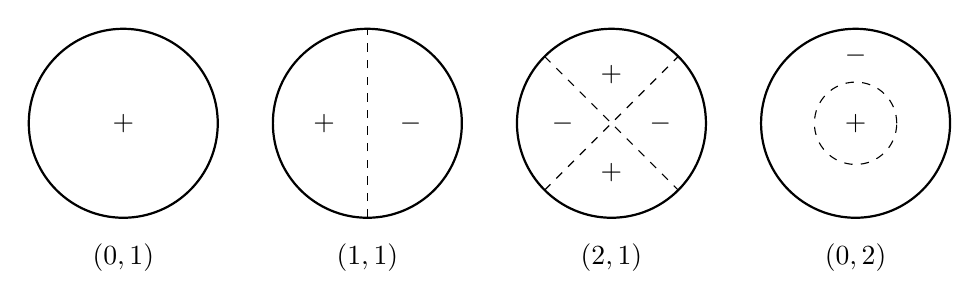
\begin{tikzpicture}
% Mode (0,1)
\begin{scope}
	\draw[thick] (0,0) circle (1.2);
	\node at (0,0) {$+$};
	\node at (0,-1.7) {$(0,1)$};
\end{scope}
% Mode (1,1)
\begin{scope}[xshift=3.1cm]
	\draw[thick] (0,0) circle (1.2);
	\draw[dashed] (0,-1.2) -- (0,1.2);
	\node at (-0.55,0) {$+$};
	\node at (0.55,0) {$-$};
	\node at (0,-1.7) {$(1,1)$};
\end{scope}
% Mode (2,1)
\begin{scope}[xshift=6.2cm]
	\draw[thick] (0,0) circle (1.2);
	\draw[dashed] (-0.849,-0.849) -- (0.849,0.849);
	\draw[dashed] (-0.849,0.849) -- (0.849,-0.849);
	\node at (0,0.62) {$+$};
	\node at (0,-0.62) {$+$};
	\node at (-0.62,0) {$-$};
	\node at (0.62,0) {$-$};
	\node at (0,-1.7) {$(2,1)$};
\end{scope}
% Mode (0,2)
\begin{scope}[xshift=9.3cm]
	\draw[thick] (0,0) circle (1.2);
	\draw[dashed] (0,0) circle (0.523);
	\node at (0,0) {$+$};
	\node at (0,0.86) {$-$};
	\node at (0,-1.7) {$(0,2)$};
\end{scope}
\end{tikzpicture}
\caption{Die vier tiefsten Schwingungsmoden der kreisförmigen Membran.
Der erste Index $n$ zählt die Knotendurchmesser und stammt aus dem Winkelanteil $\cos n\varphi$, der zweite Index $m$ nummeriert die Nullstelle $j_{n,m}$ und bestimmt die Zahl der Knotenkreise im Innern.
Die gestrichelten Linien sind die Knotenlinien, die Vorzeichen geben die Phase der Auslenkung an.
Der innere Knotenkreis der Mode $(0,2)$ liegt bei $j_{0,1}/j_{0,2}\approx 0.436$ des Radius.
Die Frequenzen verhalten sich nach \eqref{bessel:eigenschaften:eqn:eigenfrequenzen} wie $1 : 1.593 : 2.136 : 2.295$.
\label{bessel:eigenschaften:fig:moden}}
\end{figure}
 
%
% Orthogonalität
%
\subsection{Orthogonalität
\label{bessel:eigenschaften:subsection:orthogonalitaet}}
Wie die trigonometrischen Funktionen bilden auch die Bessel-Funktionen ein Orthogonalsystem, allerdings mit einer Gewichtsfunktion.
 
\begin{satz}
\label{bessel:eigenschaften:satz:orthogonalitaet}
Sind $j_{\nu,m}$ und $j_{\nu,l}$ Nullstellen von $J_\nu$, so gilt
\begin{equation}
\int_0^1
J_\nu(j_{\nu,m}s)\,
J_\nu(j_{\nu,l}s)\,
s\,ds
=
\begin{cases}
0 & \text{für } m\ne l,\\[3pt]
\dfrac{1}{2}\,J_{\nu+1}(j_{\nu,m})^2 & \text{für } m=l.
\end{cases}
\label{bessel:eigenschaften:eqn:orthogonalitaet}
\end{equation}
\end{satz}

\begin{proof}
Wir schreiben $\alpha=j_{\nu,m}$ und $\beta=j_{\nu,l}$ sowie $u(s)=J_\nu(\alpha s)$ und $v(s)=J_\nu(\beta s)$.
Setzt man $x=\alpha s$ in~\eqref{bessel:loesung:eqn:bessel} ein und dividiert durch $s$, so erhält man wegen $su''+u'=(su')'$ die selbstadjungierte Form
\begin{equation}
(s\,u')'
+
\Bigl(\alpha^2 s - \frac{\nu^2}{s}\Bigr) u
=
0,
\label{bessel:eigenschaften:eqn:selbstadjungiert}
\end{equation}
und entsprechend für $v$ mit $\beta$ anstelle von $\alpha$.

Multipliziert man~\eqref{bessel:eigenschaften:eqn:selbstadjungiert} mit $v$, die Gleichung für $v$ mit $u$ und subtrahiert, so heben sich die Terme mit $\nu^2/s$ weg und es bleibt
\[
v\,(s\,u')' - u\,(s\,v')'
+
(\alpha^2-\beta^2)\,s\,uv
=
0 .
\]
Der erste Teil ist eine vollständige Ableitung, denn es gilt
$v(su')'-u(sv')' = \frac{d}{ds}\bigl[s(u'v-uv')\bigr]$.
Integration über $[0,1]$ liefert deshalb
\[
\Bigl[\,s\bigl(u'(s)v(s)-u(s)v'(s)\bigr)\Bigr]_0^1
+
(\alpha^2-\beta^2)
\int_0^1 s\,u(s)v(s)\,ds
=
0 .
\]
Am unteren Rand verschwindet die Klammer.
Für $\nu>0$ verschwinden $u$ und $v$ nach~\eqref{bessel:loesung:eqn:kleinx} bei $s=0$ wie $s^{\nu}$ und ihre Ableitungen wie $s^{\nu-1}$, der ganze Ausdruck ist daher von der Ordnung $s^{2\nu}$.
Für $\nu=0$ sind $u$ und $v$ bei $s=0$ beschränkt, und nach~\eqref{bessel:eigenschaften:eqn:j0strich} verschwinden $u'$ und $v'$ dort wie $s$, der Ausdruck ist daher von der Ordnung $s^2$.
Am oberen Rand verschwindet sie, weil $\alpha$ und $\beta$ Nullstellen von $J_\nu$ sind und damit $u(1)=v(1)=0$ gilt.
Für $m\ne l$ ist $\alpha^2\ne\beta^2$, und es folgt die behauptete Orthogonalität.

Für $m=l$ multiplizieren wir~\eqref{bessel:eigenschaften:eqn:selbstadjungiert} mit $2su'$ und erhalten
\[
\frac{d}{ds}\bigl[(s\,u')^2\bigr]
+
(\alpha^2s^2-\nu^2)\,\frac{d}{ds}\bigl[u^2\bigr]
=
0 .
\]
Integration über $[0,1]$ und partielle Integration des zweiten Terms ergeben
\[
2\alpha^2
\int_0^1 s\,u(s)^2\,ds
=
\Bigl[\,(s\,u')^2 + (\alpha^2s^2-\nu^2)u^2\,\Bigr]_0^1 .
\]
Am unteren Rand verschwinden beide Summanden wieder, für $\nu>0$ mit der Ordnung $s^{2\nu}$ und für $\nu=0$ mit der Ordnung $s^2$.
Mit $u'(1)=\alpha J_\nu'(\alpha)$ bleibt
\[
\int_0^1 s\,J_\nu(\alpha s)^2\,ds
=
\frac{1}{2}\,J_\nu'(\alpha)^2 .
\]
Schliesslich ist $J_\nu(\alpha)=0$, aus~\eqref{bessel:eigenschaften:eqn:dreiterm} folgt deshalb $J_{\nu-1}(\alpha)=-J_{\nu+1}(\alpha)$, und~\eqref{bessel:eigenschaften:eqn:ableitungrek} liefert
\[
2J_\nu'(\alpha)
=
J_{\nu-1}(\alpha)-J_{\nu+1}(\alpha)
=
-2J_{\nu+1}(\alpha).
\]
Einsetzen ergibt die behauptete Normierung.
\end{proof}
 
Das Gewicht $s$ im Integral ist kein Schönheitsfehler, sondern das Flächenelement der Polarkoordinaten, $dA = r\,dr\,d\varphi$.
Die Orthogonalität ist also die natürliche Orthogonalität auf der Kreisscheibe.
 
Daraus ergibt sich die \emph{Fourier-Bessel-Reihe}.
\index{Fourier-Bessel-Reihe}%
Eine auf $[0,1]$ hinreichend gutartige Funktion $f$ lässt sich als
\begin{equation}
f(s)
=
\sum_{m=1}^{\infty}
c_m J_\nu(j_{\nu,m}s),
\qquad
c_m
=
\frac{2}{J_{\nu+1}(j_{\nu,m})^2}
\int_0^1 f(s)\,J_\nu(j_{\nu,m}s)\,s\,ds,
\label{bessel:eigenschaften:eqn:fourierbessel}
\end{equation}
entwickeln.
Damit lassen sich Anfangsbedingungen einer kreisförmigen Membran nach Eigenmoden zerlegen, genau wie eine Fourier-Reihe das für die Saite leistet.
 
%
% Asymptotisches Verhalten
%
\subsection{Asymptotisches Verhalten
\label{bessel:eigenschaften:subsection:asymptotik}}
Für grosse Argumente werden die Bessel-Funktionen fast zu trigonometrischen Funktionen.
 
\begin{satz}
\label{bessel:eigenschaften:satz:asymptotik}
Für $x\to\infty$ gilt
\begin{align}
J_\nu(x)
&=
\sqrt{\frac{2}{\pi x}}
\cos\Bigl(x-\frac{\nu\pi}{2}-\frac{\pi}{4}\Bigr)
+
O(x^{-3/2}),
\label{bessel:eigenschaften:eqn:asymptotikj}
\\
Y_\nu(x)
&=
\sqrt{\frac{2}{\pi x}}
\sin\Bigl(x-\frac{\nu\pi}{2}-\frac{\pi}{4}\Bigr)
+
O(x^{-3/2}).
\label{bessel:eigenschaften:eqn:asymptotiky}
\end{align}
\end{satz}

Die im Beweis von Satz~\ref{bessel:eigenschaften:satz:nullstellen} hergeleitete Normalform~\eqref{bessel:eigenschaften:eqn:normalform} macht diese Aussage verständlich.
Der Störterm $(\frac14-\nu^2)/x^2$ verschwindet für $x\to\infty$, und übrig bleibt die gewöhnliche Schwingungsgleichung $u''+u=0$.
Die Lösung ist also asymptotisch eine Schwingung der Kreisfrequenz eins, und der Faktor $1/\sqrt{x}$ kommt von der Rücksubstitution $y=x^{-1/2}u$.

Dieses Argument liefert die Gestalt der Asymptotik, aber nicht die beiden Konstanten.
Sie lassen sich an einem Sonderfall ablesen.
Für $\nu=\frac12$ ist $\frac14-\nu^2=0$, die Normalform lautet dann exakt $u''+u=0$, und die Asymptotik ist keine Näherung mehr, sondern eine Identität.
Tatsächlich gilt
\begin{equation}
J_{1/2}(x)
=
\sqrt{\frac{2}{\pi x}}\,\sin x ,
\label{bessel:eigenschaften:eqn:jhalb}
\end{equation}
wie man durch Einsetzen von $\nu=\frac12$ in die Reihe~\eqref{bessel:loesung:eqn:jnu} und Vergleich mit der Sinusreihe bestätigt.
Setzt man $\nu=\frac12$ in~\eqref{bessel:eigenschaften:eqn:asymptotikj} ein, so ist das Phasenargument $x-\frac{\pi}{4}-\frac{\pi}{4}=x-\frac{\pi}{2}$, und wegen $\cos(x-\frac{\pi}{2})=\sin x$ stimmt die Formel exakt mit~\eqref{bessel:eigenschaften:eqn:jhalb} überein.
Damit sind sowohl die Amplitude $\sqrt{2/\pi}$ als auch der Phasenanteil $-\pi/4$ festgelegt.

Der verbleibende Phasenanteil $-\nu\pi/2$ lässt sich ebenfalls kontrollieren.
Leitet man die Asymptotik von $x^{-\nu}J_\nu$ ab und vergleicht mit~\eqref{bessel:eigenschaften:eqn:ableitung2}, so verschiebt jeder Schritt von $\nu$ auf $\nu+1$ die Phase um genau $\pi/2$.
Ein vollständiger Beweis für beliebiges $\nu$ verlangt eine echte asymptotische Analyse.
Für ganzzahliges $\nu=n$ leistet das die Methode der stationären Phase, angewandt auf die Integraldarstellung~\eqref{bessel:eigenschaften:eqn:integral}, für allgemeines $\nu$ braucht man eine Integraldarstellung, die auch für nicht ganzzahlige Ordnung gilt.
Die Einzelheiten finden sich bei \cite{bessel:watson} und \cite{bessel:dlmf}.

Die Lösung ist also asymptotisch eine Schwingung, und der Faktor $1/\sqrt{x}$ kommt von der Rücksubstitution.
 
Die Abklingrate $1/\sqrt{x}$ ist physikalisch einleuchtend.
Eine von einem Punkt ausgehende Kreiswelle verteilt ihre Energie auf einen Kreis mit Umfang $2\pi r$, die Energiedichte fällt also wie $1/r$ und die Amplitude wie $1/\sqrt{r}$.
Wirft man einen Stein ins Wasser, sieht man genau das.
 
Zusammen mit~\eqref{bessel:loesung:eqn:kleinx} ist das Verhalten von $J_\nu$ damit in beiden Grenzfällen bekannt.
Nahe null verhält es sich wie eine Potenz $x^\nu$, weit draussen wie eine gedämpfte Kosinusschwingung.
Der Bereich dazwischen ist der interessante, und dort hilft nur die Reihe oder die Numerik.